% Clase 4 — Introducción a CSP
% Lectura: AIMA Cap. 5
\section{Problemas de Satisfacción de Restricciones (CSP)}

\begin{definition}[CSP]
Un CSP se define por:
\begin{itemize}
    \item $X = \{X_1, \ldots, X_n\}$: variables
    \item $D = \{D_1, \ldots, D_n\}$: dominios de cada variable
    \item $C$: conjunto de restricciones sobre subconjuntos de variables
\end{itemize}
La \textbf{solución} es una asignación completa y consistente.
\end{definition}

\subsection{Tipos de Restricciones}

\begin{itemize}
    \item \textbf{Unarias}: $X_i \in \{v_1, v_2\}$
    \item \textbf{Binarias}: $X_i \neq X_j$
    \item \textbf{Globales}: involucran más de 2 variables (ej. \texttt{AllDiff})
\end{itemize}

\subsection{Búsqueda con Retroceso (Backtracking)}

Asigna valores a variables una por una; retrocede cuando se viola una restricción.

\textbf{Heurísticas para mejorar el backtracking}:
\begin{enumerate}
    \item \textbf{MRV} (Minimum Remaining Values): elegir la variable con menos valores posibles.
    \item \textbf{Degree heuristic}: variable con más restricciones sobre variables no asignadas.
    \item \textbf{Least Constraining Value}: valor que deja más opciones para las demás variables.
\end{enumerate}

\begin{example}[Coloreado de un mapa]
    Cuatro regiones $W, X, Y, Z$ deben colorearse con $\{$rojo, verde, azul$\}$ de modo que regiones vecinas tengan
    colores distintos. Las adyacencias son: $W$-$X$, $W$-$Y$, $X$-$Y$, $X$-$Z$, $Y$-$Z$.
\end{example}

\begin{figure}[H]
\centering
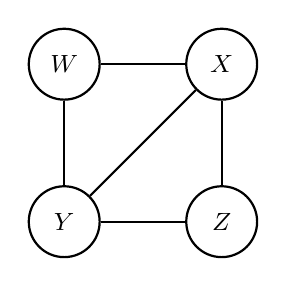
\begin{tikzpicture}[
  var/.style={draw=black, thick, circle, minimum size=9mm, font=\small}
]
\node[var] (W) at (0,2)   {$W$};
\node[var] (X) at (2,2)   {$X$};
\node[var] (Y) at (0,0)   {$Y$};
\node[var] (Z) at (2,0)   {$Z$};

\draw[thick] (W) -- (X);
\draw[thick] (W) -- (Y);
\draw[thick] (X) -- (Y);
\draw[thick] (X) -- (Z);
\draw[thick] (Y) -- (Z);
\end{tikzpicture}
\caption{Grafo de restricciones del CSP: cada nodo es una variable (región) y cada arista es una restricción binaria
de desigualdad con su vecina. $X$ y $Y$ tienen grado 3 (las más restringidas); son buenas candidatas para asignar
primero según la heurística de grado.}
\end{figure}
